\documentclass[Rapport/Rapport_main.tex]{subfiles}
\begin{document}
\subsection{Systemsekvensdiagrammer}
I dette afsnit vises de sekvensdiagrammer for systemet, der tager udgangspunkt i Use Cases \ref{sec:rap_use_cases}. Det vil sige der gennemgås de forskellige brugsscenarier for systemet. De forskellige Use Cases gennemgås i kronologisk rækkefølge.

\subsubsection{Systemsekvensdiagram for UC1: Start Spil}
Startes der med den første Use Case, \textsc{UC1: Start Spil}, så omhandler den hvordan et spil startes. Sekvensen for denne Use Case ses i figur \ref{fig:rap_sd_UC1}.
\begin{figure}[H]
    \centering
    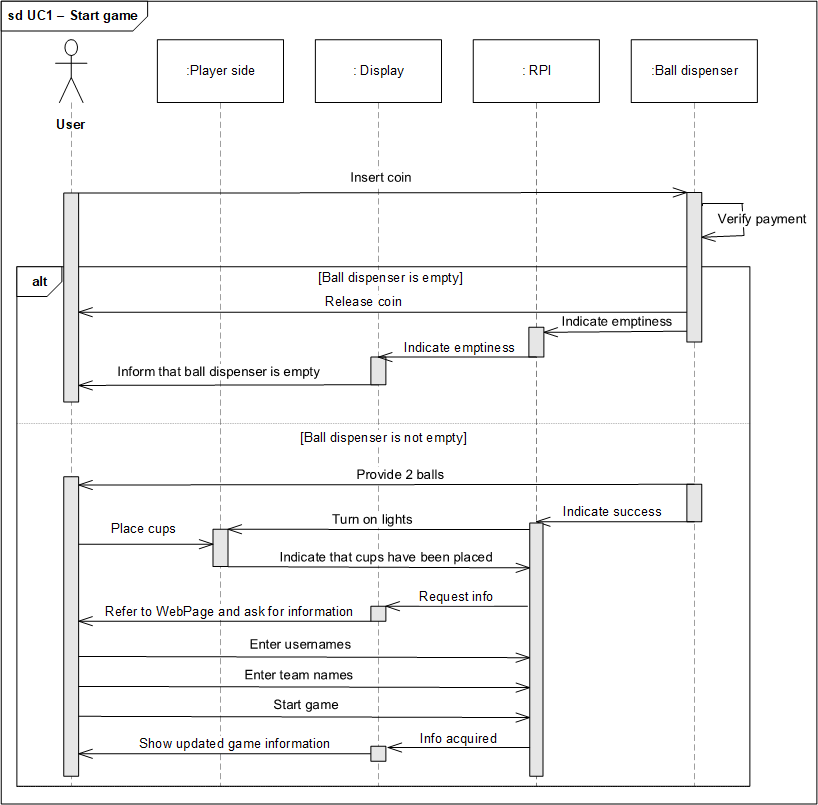
\includegraphics[width=\textwidth]{Arkitektur/Sekvensdiagrammer/graphics/sd_UC1.png}
    \caption{Systemsekvensdiagram for UC1 - Start spil}
    \label{fig:rap_sd_UC1}
\end{figure}

\subsubsection{Systemsekvensdiagram for UC2: Spil Tur}
Sekvensen for \textsc{UC2: Spil tur} bekriver spillets gang og overdragelse af \textit{\textbf{turen}}.
\begin{figure}[H]
    \centering 
    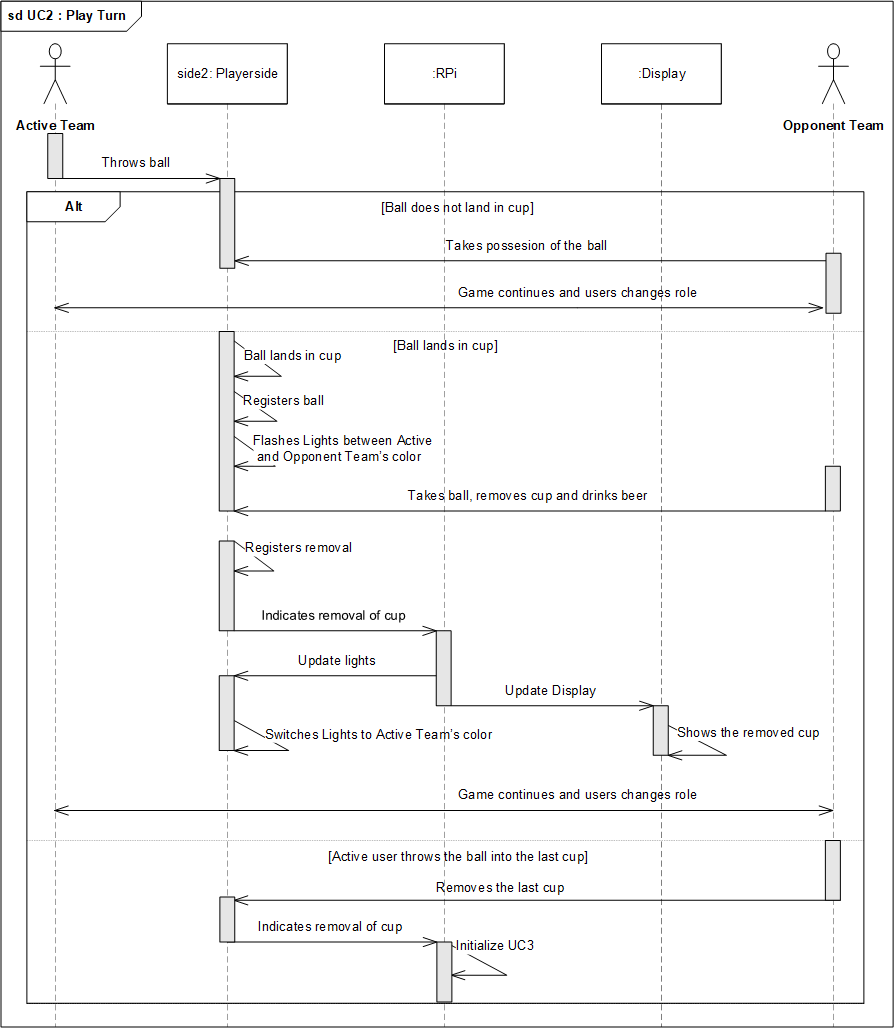
\includegraphics[width=\textwidth]{Arkitektur/Sekvensdiagrammer/graphics/sd_UC2.png}
    \caption{Systemsekvensdiagram for UC2 - Play Turn}
    \label{fig:rap_sd_UC2}
\end{figure}

\subsubsection{Systemsekvensdiagram for UC3: Afslut Spil}
For \textsc{UC3: Afslut Spil} så kan denne sekvens læses som sekvensen, der køres når et hold har tabt. Denne ses i figur \ref{fig:rap_sd_UC3}
\begin{figure}[H]
    \centering 
    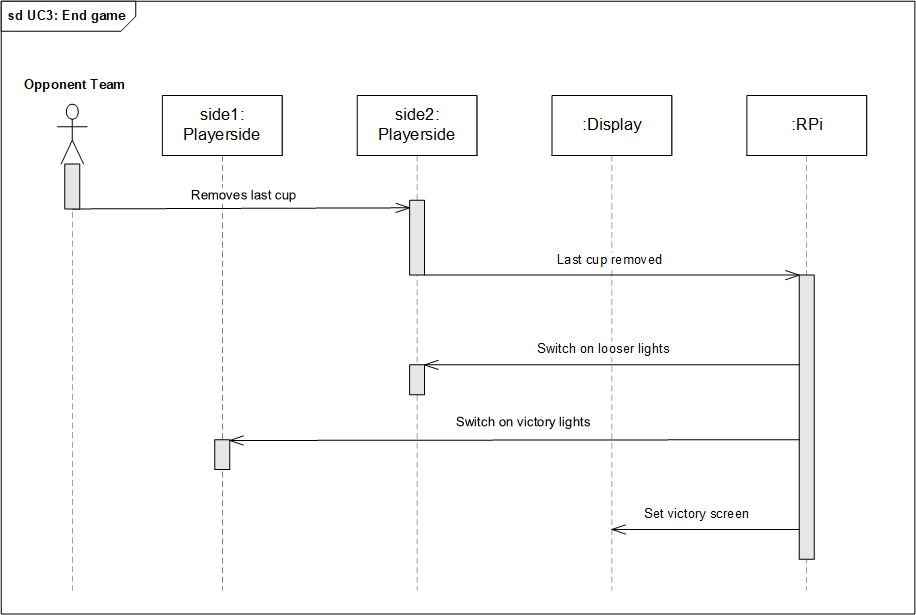
\includegraphics[width=\textwidth]{Arkitektur/Sekvensdiagrammer/graphics/sd_UC3.png}
    \caption{Systemsekvensdiagram for UC3 - End Game}
    \label{fig:rap_sd_UC3}
\end{figure}
I figur \ref{fig:rap_sd_UC3} antages der, at Opponent Team taber spillet på side 2, men det behøver ikke at være side2. Man kan i denne tilfælde godt bytte rundt med side1 og side2 uden at det påvirker sekvensdiagrammet.

\subsubsection{Systemsekvensdiagram for UC4: Påfyld Bolde}
Sekvensen for \textit{UC4: Påfyld bolde} er den service funktion, hvor en medarbejder påfylder bolde på systemet. Denne kan ses i figur \ref{fig:rap_sd_UC4}.
\begin{figure}[H]
    \centering
    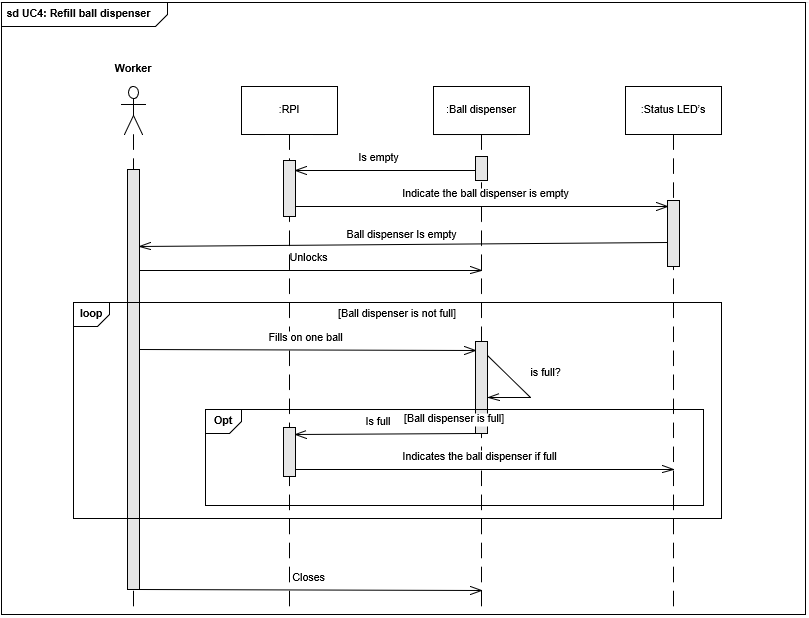
\includegraphics[width=\textwidth]{Arkitektur/Sekvensdiagrammer/graphics/sd_UC4.png}
    \caption{Systemsekvensdiagram for use case 4: Påfyld bolde}
    \label{fig:rap_sd_UC4}
\end{figure}

\end{document}